\chapter{Introduction}

\section{Problem}
(Could I just say models, here instead of generative models?)
\begin{itemize}
  \item Real world data if often causesed by multiple sources, that is independant sources combining to form data.  This creates noise and obscures part of the data we are interested in.
  \item Generative Models used in Machine learning do not capture these source independantly, meaning prior knowledge about the data is being lost(To much of a sweeping statement?). Instead the generative models are trained to learn the complex combination of data caused by the sources.
  \item Generative Model that do account for multiple sources are desirable, as the causes are encoded separately, which would(should this just be allows?) allow source separation. That is, taking a noisy input and encoding that into separate representations for each source.
  \item When the model treats sources naively, more work on data preprocessing and cleaning is needed, which often takes longer that the machine learning task itself.
  \item Frean, Marsland propose a new Generative Model that can capture two causes combining to form data, effectively encoding prior knowlege into the architecture of the model.
  \begin{itemize}
    \item It builds on and combines previous work on Restricted Boltzmann Machines and Sigmoid Belief Networks.
    \item The theory had been checked but the new model had not been tried in practice. Frean and Marsland needed confidence around some key areas
    \begin{itemize}
      \item Can this model encode a multi-cause input(need to define this?) as separate causes?
      \item How does the time-efficiency of this model compare to the standard Restricted Boltzmann machine?
      \item (Do I want to talk about learning?)
    \end{itemize}
    \item These are non-trivial tasks as the Restricted Boltzmann Machine, and the proposed model that uses it, are stochastic unsupervised learners making evaluation non-trivial. We cannot simply inspect the representations generated in the new model.
    \item There is(was?) a need to implement this new approach and then verify that it can or cannot perform source separation.
  \end{itemize}
\end{itemize}

\section{Solution}

\begin{itemize}
  \item This project answered(answers?) these questions, evaluating the new generative model by way of experimentation. The ablility for the new generative model (I really need a name for this)  to separate the sources has been evaluated on various sizes (better word here) of problems.
\end{itemize}

To describe the new generative model proposed and explored in this report some concepts must be introduced.

\section{Probablistic Graphical Models}

Probalistic Graphical Models or PGMs for short, are an expressive way to represent a model with dependancies and probabilities associated with different states. TODO-CITE-DAVID-BARBERS-TEXTBOOK-ON-PGM-USE.

\section{Generative Models}

Generative models are a powerful way to model data. In the context of images, generative models, if trained, can randomly generate observable data.
The generative model proposed in this project aims to represent data generated by two causes.

  \subsection{Training Generative Models}
  \begin{itemize}
    \item Training generative models with some param big theta, gradient amounts to log likelihood of dataset minus normalisation.
    \item Amounts to hebbain learning. Reasoned about by Donald Hebb, connections between neurons in the brain during learning, the more often a memory is accessed or used, the strong the connection it should make
    \item Wake phase
    \item Sleep phase
  \end{itemize}

\section{Sampling}

Sampling is the process of drawing samples from a distribution. It is used when the distrubtion we want samples from is intractable to calculate
analytically. Sampling is required to train generative models, as often the gradient to be climbed/descended involves calculating a probability in the
generative model.

\begin{itemize}
  \item Inference is the process of given reasoning about what we do not know given that of which we do know.
  \item In a Generative Model this amounts to the Posterior
\end{itemize}

  \subsection{Markov Chain}

  \begin{itemize}
    \item The importance of Markov Chains and mixing time are crutial in this project
  \end{itemize}


  \subsection{Gibbs Sampling}

  Gibbs sampling is a special case of Markov Chain Monte Carlo, a technique for sampling from a complex distribution. The probability mass of a generative model is a common use case for Gibbs sampling.



\section{Belief Networks}

A belief network is technique of modeling causual data. The network is directed representing cause, nodes in the network represent binary variables which are dependant on ancestor nodes, the degree of which is encoded in a conditional probalitity table. The belief network provides a succint encoding of depedancies between variables. Several algorithms operate on this representation, determining the probability of a variables state, given the states of its ancestors. One of such algorithms is Belief Propagation/Sum-Product Algorithm. However this technique breaks down in larger dimensions with a cost of TODO


The technique proposed in this report relies on the parameterised version of the belief network, the Sigmoid Belief Network. The sigmoid belief network is composed of sigmoid units, akin to that of a perceptron linear threshold unit. The weighted sum of the inputs to a variable in the system is passed through a sigmoid function, the weights capturing the dependance between a node and its ancestors.

Belief Networks appear to be an intuitive way to model data in machine learning, as rich dependancies often present in real data can be expressed in its architecture. Unfortunately, due to the effect of explaining away, it is intractable to perform inference in a belief network which is needed required for training.

  \subsection{Explaining Away}

  The power of the belief network is also its weakness, a rich structure that models a system of interest inheriently has depedancies. In its minimal case explaining away can be seen in a 3 node network popularised by TODO-CITE-AI-A-MODERN-APPROACH-TODO. TODO-GRAPHIC

  In this network knowledge of the alarm creates a dependance between Burglar and Earthqaukes. For instance, say the Alarm has gone off and we know an earthquake has occurred, our belief in being burgaled decreases. The dependance in belief networks means that sampling from the network requires a longer Markov Chain to mix.

  In the context of images, where there may be upwards of 1000 observable values, all with different depedancies this is intractable.

\section{Boltzmann Machines}

A Boltzmann machine shares a few qualities with Belief Networks. Both are generative models, and variables/nodes have probabilities of being active/deactive based on neighbouring nodes. Unlike a Belief Network, a Boltzmann Machine is a undirected network meaning connections between nodes no longer encode causal information. Performing gibbs sampling appears trivial in a Boltzmann Machine, in that to find the probability of a given unit being active a weighted input to that node is passed through a sigmoid function. However, in practice the recurrent nature of Boltzmann Machines makes sampling intractable.

TODO-REFENCE-PAPER-OF-THIS The Boltzmann Machine was shown, given an unreasonable amount of time, to be able to perform better than the state of the art at the time.

\section{Restricted Boltzmann Machines}

Hinton TODO-REFERENCE-THE-PAPER proposed a restriction by way of assumption to the Boltzmann Machine that makes it tractable to sample from and therefore train. Boltzmann Machines of this architecture are referred to as Restricted Boltzmann Machines, or RBMs for short.

The assumption being that the observable and latent variables are independant respectively, enforcing a two layer, fully connected bipartide structure. The affect of this being that inference can be tractably computed as the latent variables no longer become dependant given the observed variables.

  \subsection{Contrastive Divergence}
  Hinton TODO-CITE-CLASSIC-PAPER proposed Contrastive Divergence as a method for training RBMs efficiently. The algorithm leverages the now tractable wake phase because $P(h|v)$ is efficeint to compute. However the free or sleep phase required another restriction where the network is only left to its own dynamics can be limited to only one iteration and still perform well. TODO-CITE-CD-PAPER

The observed variables are often referred to as the visible units, and will be so forth in this report. The latent variables are often referred to as the hidden units, and will be so forth in this report. Therefore the Restricted Boltzmann machine transforms some visible unit into a hidden representation. These two layers of units can be thought of as vectors of binary values, referred to as $ v $ and $ h $ for visible and hidden layers respectively.

This restriction allows an efficient calculation of the Wake Phase of generative model learning, as the $ P(h|v) $ can be calculated as a simple weighted sum passed through a sigmoid followed by a bernouli trial where the probability of being $1$ is equal to the result of sigmoid.

\begin{itemize}
  \item Unrolling the gibbs chain and we are in effect training an infinite depth sigmoid beleif net TODO-REFERENCE-HINTONS-PAPER-HERE
\end{itemize}

  \subsection{Evaluating Restricted Boltzmann Machines}

  \begin{itemize}
    \item Being unsupervised makes it difficult to evaluate RBMs. Often used as part of a deeper network, feature extractor, autoencoder
    \item Hinton Diagrams allow visualisation of hidden unit utlisation TODO-SOME-SORT-OF-CITE. The weights out of a given hidden unit can be visualised in visible data space. The weights should exhibit some structure if they are being utlisied. This is a good smoke tests for non-tulised hidden units will look very similar to units with random initial weights.
    \begin{itemize}
      \item Small Cases
      \begin{itemize}
        \item  IN trivial cases an RBM can inspected analytically
        \item Hand craft weights can be used to perform inference in a 'perfect model'. For instance an RBM that can capture two bit, logical XOR can be represented as :TODO-INSERT-PIC
      \end{itemize}
    \end{itemize}
  \end{itemize}

  \begin{figure}[]
  \begin{center}
  	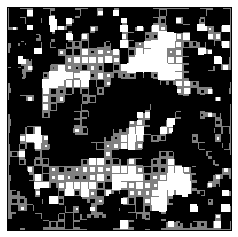
\includegraphics[]{Assets/HINTON1}
  \caption{ Good Hinton Diagram}
  \label{F:TEMP}
  \end{center}
  \end{figure}
  \begin{figure}[]
  \begin{center}
    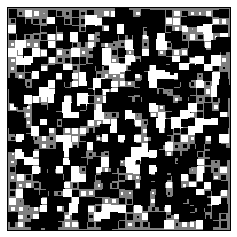
\includegraphics[]{Assets/HINTON2}
  \caption{Bad Hinton Diagram}
  \label{F:TEMP}
  \end{center}
  \end{figure}
